\section{Das Magnetische Feld}

\subsection{Energie und Kraft im magnetischen Feld}
\textbf{Energiedichte:}
$\boxed{w_m=\int_0^B{\vec{H}\cdot d\vec{B}}}$ (Allgemein)
$\qquad\boxed{w_m=\frac{1}{2}B\cdot H}$ (homog. Feld) $\qquad [w_m]=\frac{J}{m^3}$\\

\textbf{Energie:}
$\boxed{W_m = \frac{1}{2} \cdot L \cdot I^2=\frac{1}{2}\cdot N \cdot I \cdot
\Phi \; \text{ or } \; W_m=\frac{1}{2} \int_V \vec H \cdot
\vec B \cdot dV}$ (Allg.)
$\quad\boxed{W_m=w_m \cdot V=\frac{1}{2} \cdot B \cdot H \cdot V}$ (homog. Feld)\\
%\parbox{5cm}{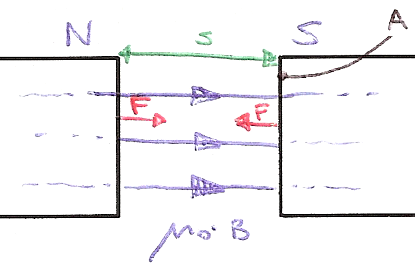
\includegraphics[width=4cm]{./pics/m-kraft-mfeld.png}}
\parbox{13cm}{	
	Die Kraft auf Grenzfl�chen ist stets so gerichtet, dass sie die Induktivit�t
	zu vergr�ssern sucht. Das heisst immer vom ferromagnetischen Material zur
	nichtferromagnetischen Umgebung (z.B. Luft). Prinzip der virtuellen
	Verschiebung:\\
	$$\boxed{F = \left| \frac{\mathrm dW_m}{\mathrm ds} \right| = \frac{1}{2} I^2 \cdot \frac{\mathrm dL}{\mathrm ds} 
	\qquad oder \qquad  F = \frac{1}{2} \cdot B \cdot H \cdot A=\frac{1}{2} \cdot
	\frac{B^2}{\mu} \cdot A \text{ (f�r } \mu_{rFe} \gg  \text{ 1)}}$$ }


\subsection{Wichtigste Formeln}

Magnetische Feldlinien verlaufen ausserhalb eines Magneten vom Nord- zum S�dpol
und sind immer geschlossen.\\ 
	\begin{tabular}[c]{ | p{5cm} | p{8cm} | p{4cm} | }
		\hline
		\textbf{Name} & \textbf{Formel} & \textbf{Einheit}\\    
		\hline
		Permeabilit�t
		& $\mu = \mu_0 \mu_r = \mu_r 4 \cdot \pi \cdot 10^{-7} \frac{Vs}{Am} = \mu_r 1.2566 \frac{\mu H}{m}=\frac{B}{H}$
		&$\frac{\mu H}{m}=\frac{Vs}{An}$\\
		& $\mu_{eff}=\frac{B}{\mu_0 H_{eff}} =
		\frac{\mu_r}{1+\mu_0\frac{l_{Luft}}{l_{FE}}}$ &\\ \hline
		Magn. Flussdichte %B = \frac{\mu}{4 \pi} \cdot \frac{Q v}{r^2} =
		& $B = \frac{F}{Q \cdot v} = H \mu \text{, wobei } \vec{v} \perp
		\vec{B}$ & $\frac{Vs}{m^2} = T$ (Tesla) \\
		\hline
		Lorentzkraft
		& $\vec{F} = Q (\vec{v} \times \vec{B})=I(\vec{l}\times \vec{B}) \hspace{1cm} |\vec{F}| = Q \cdot v \cdot B
		\cdot \sin\alpha$
		&$N$\\
		Amp�resches Gesetz
		&$F=\frac{Q_2\cdot v_2 \cdot Q_1 \cdot v_1 \cdot \mu}{r^2 \cdot 4\pi}$
		&\\
		\hline
		\textbf{3-Finger-Regel: (rechte Hand)}
		& $F$ = Daumen, $v$ = Zeigefinger, $B$ = Mittelfinger
		& Bei $Q < 0$ wechselt Richtung von B!\\
		\hline
		Magnetische Feldst�rke
		& $\vec{H} = \frac{ \vec{B}}{\mu }$
		& $\frac{A}{m}$\\
		Biot-Savart
		&$H$ (bei Punkt P) $= \frac{I}{4\pi} \int \frac{\vec{dl} \times
		\vec{r(l)}}{r^3(l)}$&\\
		& $H_{eff}= \frac{\Theta_{Ges}}{l_{FE}}$ & \\ \hline
		Magnetische Spannung
		& $V_{mAB} = \int\limits \vec{H}(s) \cdot \vec{ds}$ ($V_m$ ist abh�ngig vom
		Weg) & $A$ \\
		\hline
		Durchflutung
		& $\Theta = \oint\vec{H} \cdot \vec{ds} = \int\limits \vec{J}
		\cdot \vec{dA} \vee \underbrace{\sum I_k}_{= N I} = V_m$
		& $A$\\
		\hline
		Magnetischer Fluss
		& $\Phi = \int \vec{B} \vec{dA}$
		& $Vs = Wb$ (Weber)\\
		& $\Phi = B \cdot A \cdot \cos(\gamma)$
		& B homogen\\
		\hline
		\textbf{Maxwell-Gesetz}
		& $\oint \vec{B} \vec{dA} = 0$ (vgl. Kirchhoff 1 ($\sum I = 0$))
		&\\
		\hline
		F�llfaktor
		&$F=\frac{A_{Effektiv Fe}}{A_{Tot}}$
		& $[-]$\\
		\hline
		Magn. Widerstand
		& $R_m = \frac{V_m}{\Phi} = \frac{\Theta}{\Phi} = \frac{l}{\mu A} $
		& $\frac{A}{Wb}$ \\
		``Ohmsches	Gesetz des Magn.``
		&&\\
		\hline
		Magn. Leitwert
		& $\Lambda = \frac{1}{R_m} = \frac{\Phi}{V_m}=\frac{\Phi}{\Theta}$
		& $\frac{Vs}{A} = H$ (Henry) (Im Formelbuch als $A_L$)\\
		\hline
		Verketteter Fluss
		& $\Psi = \sum \Phi $ (meist $\Psi = N \Phi$)
		& $[\Psi] = [\Phi] = Vs = Wb$\\
		\hline
		Induktivit�t
		& $L = \frac{\Psi}{I}  \qquad \text{Bei idealer Koppl.: } L = \Lambda N^2 = \frac{N^2}{R_m} $
		& $[L] = \frac{Vs}{A} = H$\\
		\hline
		Gegeninduktivit�t
		& $M = M_{21} = M_{12}$ Bei idealer Koppl. $M = \sqrt{L_1 L_2}$
		& vorder Index = Wirkung,\\
		&$M_{21} = \frac{\Psi_{21}}{I_1}$  (meist $M_{21} = \frac{N_2 \Phi_{21}}{I_1}$)
		& hinterer = Ursache\\
		\hline
		Kopplungsfaktor
		& $k = \frac{M}{\sqrt{L_1 L_2}}$ Bei idealer Kopplung: $k = 1$
		& $[-]$ \\
		\hline
		Streukoeffizient
		& $\sigma = 1 - k^2 = 1 -\frac{M^2}{L_1 L_2}$ Bei idealer Kopplung: $\sigma = 0$
		& $[-]$\\
		\hline
		Kreis-r in M-Feld abgelenkte Q
		& $ m_e = 9,11 \cdot 10^{-31} kg$
		& $r = \frac{m_Q \cdot v}{Q \cdot B}$ \\
		\hline
	\end{tabular}
	
\subsection{Diverse Formeln bzgl. Magnetismus}
\begin{tabular}[c]{l l}
$\text{Hall-Sonde: }$
&$\text{Kraft auf stromf�hrende Leiter: }$\\ 
$U_H = \frac{I \cdot B}{e \cdot n_p \cdot h}$
&$\vec{F_L} = I (\vec{l} \times \vec{B}) \qquad F_L = I \cdot l \cdot B \cdot \sin{\alpha}$\\

Magnetfeld ausserhalb eines langen Leiters:
&Magnetfeld innerhalb eines geraden, langen Leiters: \\
$H(r) = \frac{I}{2 \cdot \pi \cdot r}$
&$H(r) = \frac{I}{2 \pi r} \frac{A_{eingeschlossen}}{A_{total}} = 
 \frac{I}{2 \pi} \frac{r}{r_a^2}$\\
Magnetfeld der Zylinderspule:
&Magnetfeld einer Toroidspule:\\
$H(r) = \frac{N \cdot I}{l}= \frac{\theta}{l} \qquad l \gg d$
& $H_{innen}(r) = \frac{N \cdot I}{2 \cdot \pi \cdot r \to l} \qquad H_{aussen}
= 0$
\end{tabular}

\begin{tabular}{llll}
\parbox{4.5cm}{
	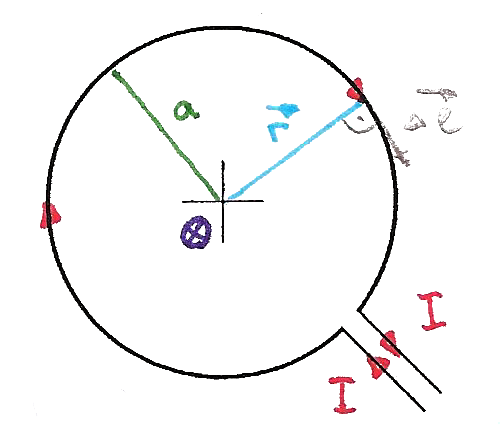
\includegraphics[width=2.7cm]{./pics/biot1.png} \\
	$H =\frac{I}{D} = \frac{I}{2a}$}
& \parbox{4.5cm}{
	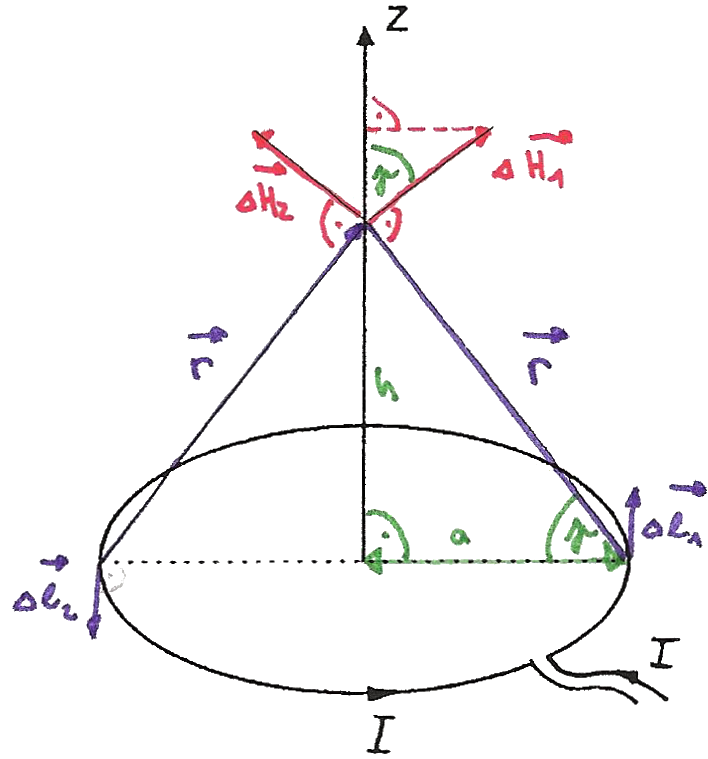
\includegraphics[width=2.7cm]{./pics/biot2.png} \\
	$H=\frac{I}{2} \cdot \frac{a^2}{\sqrt{a^2+h^2}^3}$}
& \parbox{4.5cm}{
	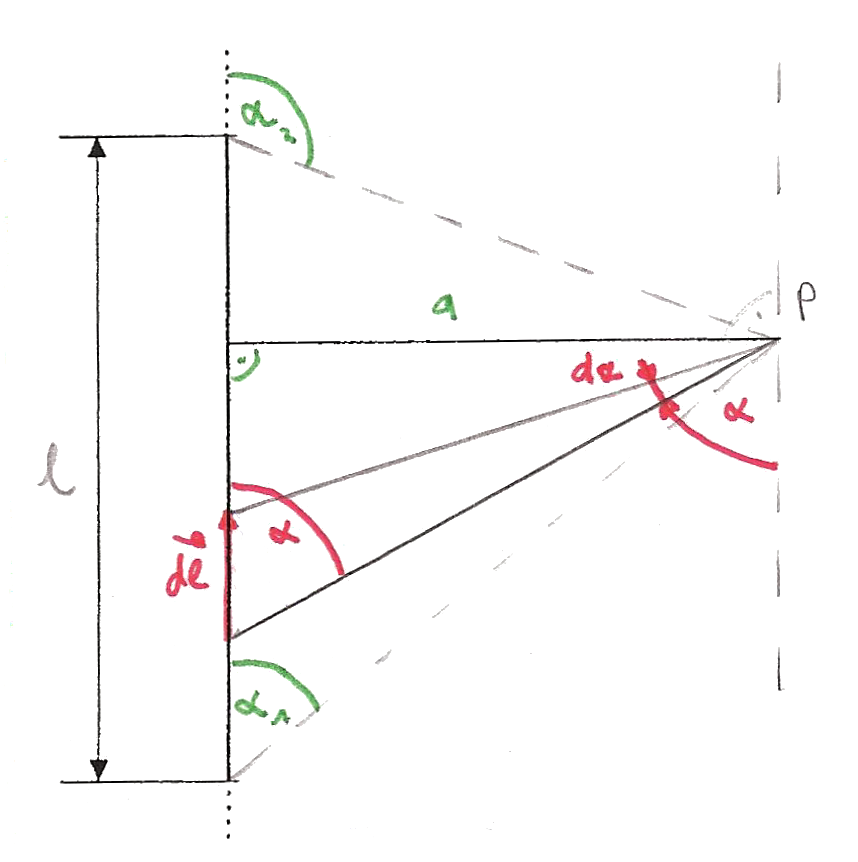
\includegraphics[width=3cm]{./pics/biot3.png} \\
	$H=\frac{I}{4\pi a}(\cos(\alpha_1)- \cos(\alpha_2))$}
& \parbox{4.5cm}{
	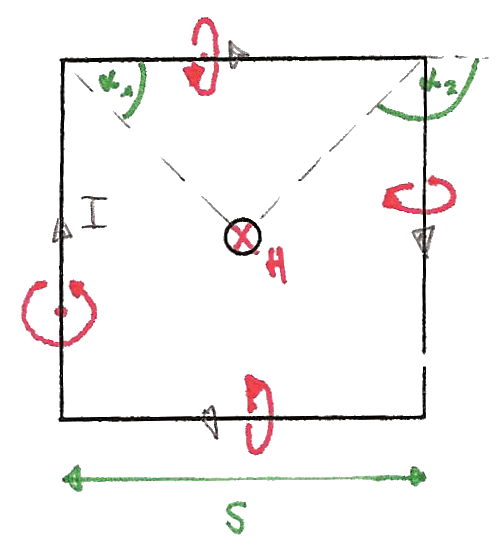
\includegraphics[width=2.7cm]{./pics/biot4.png} \\
	$H= \frac{I \cdot 2 \sqrt{2}}{\pi \cdot s}$ }
\end{tabular}

\subsection{Zusammenstellung magnetischer Gr�ssen f�r spezielle
Leiteranordnungen}
\begin{tabular}{|p{5cm}|l|l|l|l|l|}
  \hline
  & Leitwert $ \Lambda $ & Durchfl. $ \Theta $ & Fluss $ \Phi ^{1)} $ &
  Verk.-Fluss $ \Psi $ & Induktivit�t $L^{2)}$ \\
  \hline
  Kreisf�rmige Schleife & $\frac{\mu D}{2}\cdot\ln\frac{D}{d}$ & $\Theta = I$ & $\frac{\mu D}{2}\cdot\ln\frac{D}{d}\cdot I$ & $\Psi = \Phi$ & $L=\frac{\mu
  D}{2}\cdot\ln\frac{D}{d}$\\
  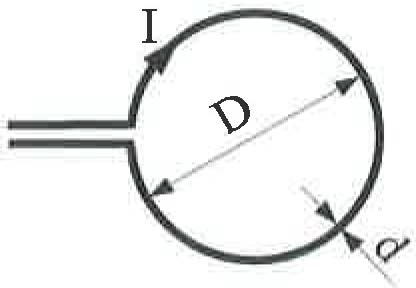
\includegraphics[width=3cm]{./pics/kreisfoermige_schleife.png} & & & & & \\
  \hline
  Kreisrahmenspule$^{3)}$ & $\frac{\mu D}{2}\cdot\ln\frac{D}{d}$ & $\Theta = NI$ & $\frac{\mu D}{2}\cdot\ln\frac{D}{d}\cdot N \cdot I$ & $\Psi = N \cdot \Phi$ & $L=\frac{\mu  D}{2}\cdot\ln\frac{D}{d}\cdot N^2$\\
  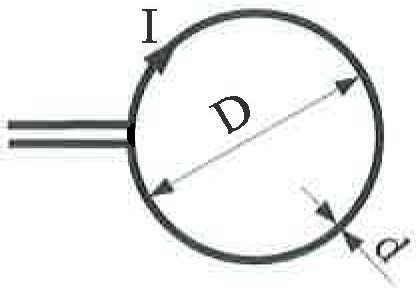
\includegraphics[width=3cm]{./pics/kreisrahmenspule.png} & & & & & \\
  \hline
  Zylinderspule $l \gg d$
  & $\frac{\mu A}{l} = \frac{\mu \pi d^2}{4l}$ & $\Theta = NI$ & $\frac{\mu \pi d^2}{4l} \cdot N \cdot I$ & $\Psi = N \cdot \Phi$ & $L=\frac{\mu \pi d^2}{4l}\cdot N^2$\\
  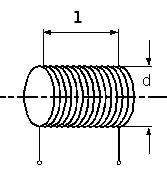
\includegraphics[width=3cm]{./pics/zylinderspule.png} & & & & & \\
  \hline
  Toroidspule $^{4)}$ & $\frac{\mu A}{l_m} = \frac{\mu d^2}{4 D_m}$ & $\Theta = NI$ & $\frac{\mu d^2}{4 D_m}\cdot N \cdot I$ & $\Psi = N
  \cdot \Phi$ & $L=\frac{\mu d^2}{4 D_m}\cdot
  N^2$\\
  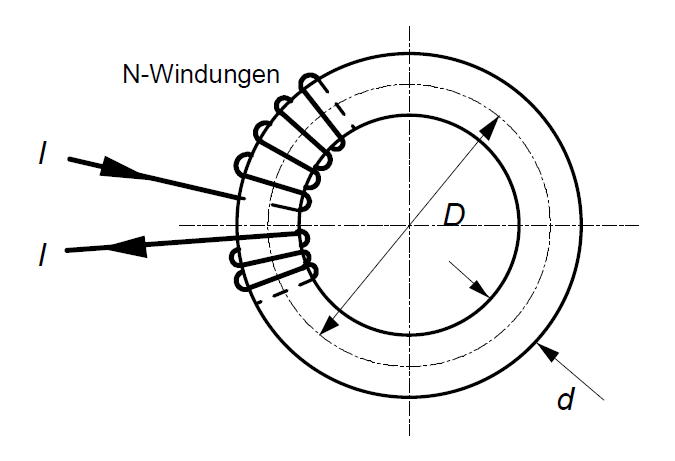
\includegraphics[width=4cm]{./pics/toroidspule.png} & & & & & \\
  \hline
  Ringspule mit rechteckf. Querschnitt & $\frac{\mu a}{2
  \pi}\cdot\ln\frac{D}{d}$ & $\Theta = NI$ & $\frac{\mu a}{2\pi}\cdot\ln\frac{D}{d}\cdot N \cdot I$ & $\Psi = N
  \cdot \Phi$ & $L=\frac{\mu a}{2\pi}\cdot\ln\frac{D}{d}\cdot N^2$\\
  \hline
  Koaxialleitung $R_2 > R_1$
  & $\frac{\mu l}{2 \pi}\cdot\ln\frac{R_2}{R_1}$ & $\Theta = I$ & $\frac{\mu l}{2\pi}\cdot\ln\frac{R_2}{R_1}\cdot I$ & $\Psi = \Phi$ & $L=\frac{\mu l}{2\pi}\cdot\ln\frac{R_2}{R_1}$ \\
  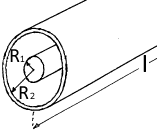
\includegraphics[width=3cm]{./pics/e-c-koaxialkabel.png} & & & & & \\
  \hline
  Paralleldrahtleitung $l \gg a \gg R$ & $\frac{\mu l}{\pi}\cdot\ln\frac{a-R}{R}$ & $\Theta = I$ & $\frac{\mu l}{\pi}\cdot\ln\frac{a-R}{R}\cdot I$ & $\Psi = \Phi$ & $L=\frac{\mu l}{\pi}\cdot\ln\frac{a-R}{R}$\\
  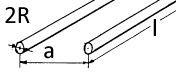
\includegraphics[width=3cm]{./pics/e-c-paralleldraht.png} & & & & & \\
  \hline
\end{tabular}

\begin{tabular}{p{8.5cm}p{8.5cm}}
  \textbf{Bemerkungen:} & \textbf{Allgemein:} \\
  $1) $ ohne Fluss durch Leiter & $\Phi = \Lambda \cdot \Theta , \Lambda =
  \frac{1}{R_m}$\\
  $2) $ nur �ussere Induktivit�t & $L=\frac{\Psi}{I}$\\
  $3) A=\frac{\pi d^2}{4}\ \ l_m \approx \pi D_m$ & $L=\Lambda=\frac{1}{R_m},
  falls N=1$ \\
  $4) $ Wickeldurchmesser d in radialer und axialer Richtung $d\ll D$ &
  $L=\Lambda N^2 =\frac{N^2}{R_m}$, falls die N-Windungen unter sich ideal
  gekoppelt sind.
\end{tabular}

\subsubsection{Ferromagnetische Stoffe}
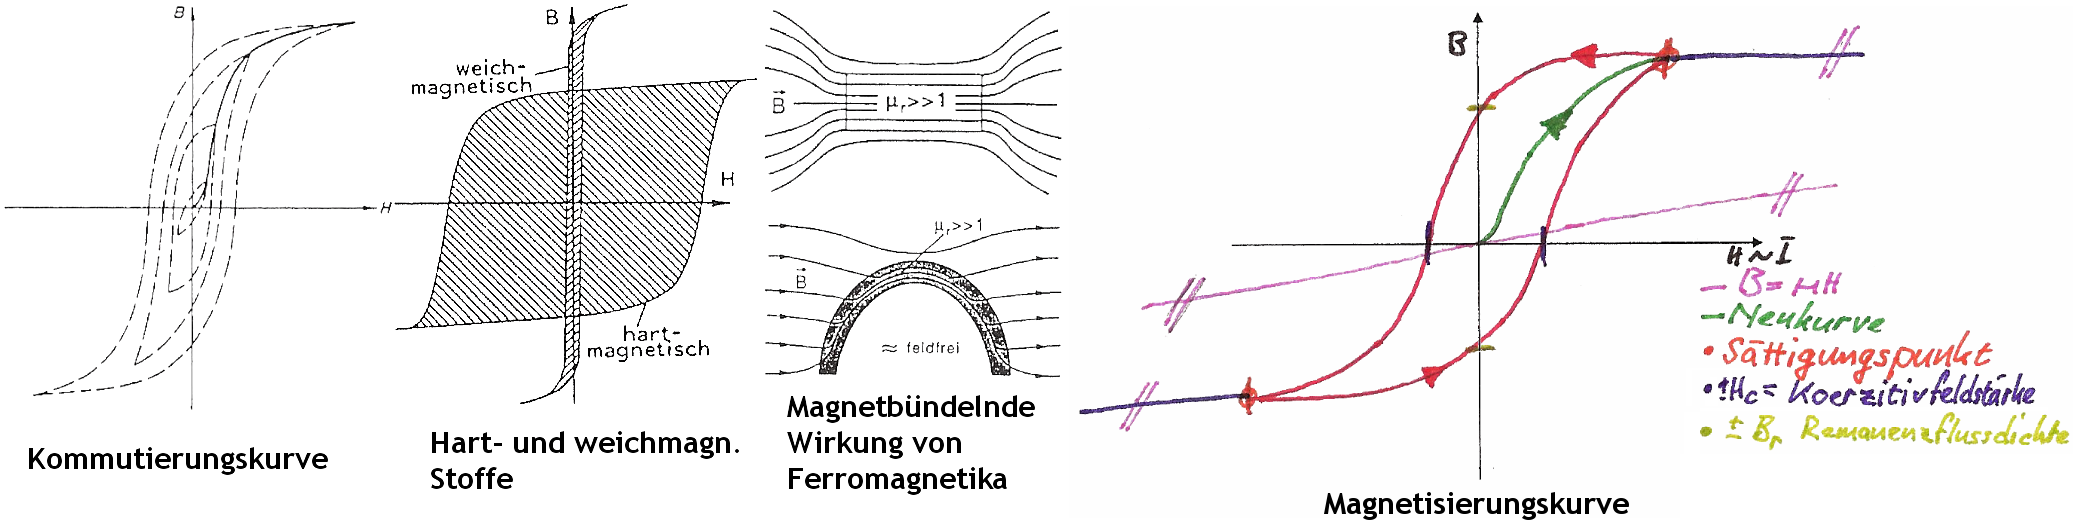
\includegraphics[width=18cm]{./pics/magnetisierung.png}
